\documentclass{article}

\usepackage[utf8]{inputenc}

\usepackage{color}
\usepackage{amsmath}
\usepackage{amsfonts}
\usepackage{amssymb}
\usepackage{amsthm}
\usepackage{mathabx}
\usepackage{geometry}
\usepackage{graphicx}
\usepackage{pgf}
\usepackage{tikz}

\geometry{
	b5paper,
	margin=1.5cm,
	top=1.75cm,
	bottom=1.75cm
}

\newcommand{\llinnm}[2]{\operatorname{L}_{\operatorname{lin}}({#1}, {#2})}
\newcommand{\llinn}[1]{\llinnm{#1}{#1}}
\newcommand{\hlinr}[1]{\operatorname{H}_{\operatorname{lin}}^{#1}}
\newcommand{\hlin}{\operatorname{H}_{\operatorname{lin}}}
\newcommand{\leap}[3]{\operatorname{\mathbf{leap}}({#1}, {#2}, {#3})}
\newcommand{\hfact}[2]{\operatorname{H}_{\operatorname{factor}}({#1}, {#2})}
\newcommand{\rot}[2]{\operatorname{H}_{\operatorname{rot}}^{{#1}, {#2}}}

\newcommand{\bin}[3]{\operatorname{\mathbf{bin}}({#1}, {#2}, {#3})}
\newcommand{\lbin}[2]{\operatorname{\mathbf{lbin}}({#1}, {#2})}

\newcommand{\vecspace}[2]{\mathbb{Z}_{#1}^{#2}}
\newcommand{\binvecspace}[1]{\vecspace{2}{#1}}
\newcommand{\linearmaps}[2]{\mathcal{L}_{#1}^{#2}}
\newcommand{\surjectivelinearmaps}[2]{\mathcal{LS}_{#1}^{#2}}

\newcommand{\probs}[2]{\operatorname{\mathbf{Pr}}_{{#1}}\left[{#2}\right]}
\newcommand{\prob}[1]{\probs{}{#1}}
\newcommand{\expects}[2]{\operatorname{\mathbf{E}}_{{#1}}\left[{#2}\right]}
\newcommand{\expect}[1]{\expects{}{#1}}
\newcommand{\inu}{\in_U}

\newtheorem{lemma}{Lemma}
\newtheorem{definition}{Definition}
\newtheorem{theorem}{Theorem}
\newtheorem{claim}{Claim}
\newtheorem{corollary}{Corollary}

\title{An upper bound on the size of the largest bin using linear transformations over vector spaces}

\author{Martin Babka}

\begin{document}

\maketitle

\begin{abstract}
We estimate the expected size of a largest bin when hashing $n$ balls into $n$ bins using matrix multiplication, i.e. functions of the form $Ax + b$ where $A$ is a binary matrix and $b$ is a binary vector.
The currently known upper bound for this settings is $O(\log n \log \log n)$ by Alon et al. and holds for hashing $n \log n$ balls into $n$ bins.
We show an estimate for placing $n$ balls into $n$ bins and get $O(\log n)$ estimate on the size of the largest bin.
The bound is proven using the same technique but using different parametrization.
\end{abstract}

\section{Introduction}

Nowadays the research is focused on finding the as fast as possible hash function families with small largest bins.
Placing balls with small largest bins have applications for example in load balancing, plain universal hashing and many others.
The best possible bound for families of hash functions mapping arbitrary subset of the given universe is $O(\log n/\log \log n)$ and can be achieved by various systems.
If the system is at least $\log n/\log \log n$-independent, then the above bound is achieved.
However systems with high independence are inefficient in practice because of size and/or speed according to Siegel's lower bound~\cite{siegel}. 
The research moved from finding highly independent systems to finding functions which best fit the needs of the application. 

Small systems specially designed to achieve the optimal sublogaritmic bound emerged in \cite{celisetal}.
There are also other settings such as cuckoo hashing, linear probing, etc. and there are special designs of hash function systems which accommodate to the special needs of these settings.
For cuckoo hashing there are known families and modifications which keep the expected $O(1)$ operation time, for example using stash and hashing functions from \cite{mitzenmacher-cuckoo} and \cite{dietzfelbinger-cuckoo}.
For linear probing it is known that 5-indepence is enough to achieve the expected constant probe sequence length~\cite{linear-probing}.
For all the above applications $O(\log n)$ independence is sufficient to have expected $O(1)$ insertion time or expected constant probe sequence length.

In this article we are bounding the size of a largest bin without having large independence.
We asymptotically improve a known estimate on the size of the largest bin for the system of linear transformations.
The linear transformations between the binary vector spaces form a simple natural two-wise independent system of functions.
We assume that $n = 2^b$ and we have $n$ elements arbitrarily chosen from the universe $\binvecspace{u}$.
If they are placed into the table of size $n$ using a randomly chosen linear transformation from $\binvecspace{u}$ to $\binvecspace{b}$, then the expected size of a largest bin is $O(\log n)$.
As already mentioned for two-wise independent systems it is apriori not known whether the expected size of a largest bin is polylogarithmic with respect to the number of placed elements.
Especially for the system of linear mappings it has been already shown in a paper by Alon et al \cite{alonetal} that the bound is $O(\log n \log \log n)$ for placing $n \log n$ balls into $n$ bins.
This bound certainly holds for placing $n$ balls into the same number of bins.
In this paper we improve this bound by $\log \log n$ factor when assuming that just $n$ balls are placed into the same number of bins.

The technique of the proof is similar as in the original proof. We switch to a different parametrization and change a few statements so that they fit to the current setting.
Our result is still not known and the asymptotic improvement has impact on hashing using linear functions.
For example storing sets using hashing with linear functions now matches the asymptotic bounds achieved by balanced trees.

\section{Setting and notation}
Let $u, b \in \mathbb{N}$ and let $A$ be a binary matrix of dimension $u \times b$, i.e. $A \in \{0, 1\}^{u \times b}$, and $a \in \{0, 1\}^b$, by linear transformation from $\binvecspace{u}$ to $\binvecspace{b}$ we understand a mapping $x \mapsto Ax + a$.
By $\linearmaps{u}{b}$ we denote all linear transformations from the vector space $\binvecspace{u}$ to $\binvecspace{b}$.
By $\surjectivelinearmaps{u}{b}$ we denote all surjective linear transformations from $\binvecspace{u}$ onto $\binvecspace{b}$.
Let $S \subseteq \binvecspace{u}$ and $T \in \linearmaps{u}{b}$, then by $\lbin{T}{S}$ we denote the size of the largest bin created by $T$ when hashing $S$, i.e. $\lbin{T}{S} = \operatorname{argmax}_{y \in \binvecspace{b}} |T^{-1}(y) \cap S|$.
In the article the dimension of the universe is always $u$, the set of placed balls is denoted by $S$, $S \subseteq U$.

\section{Placement of $n$ Balls into $n$ Bins}

Throughout this section we assume placement of $n$ balls into $n$ bins using linear transformations.
Moreover we assume that $n = 2^b$ for a positive integer $b$.
\begin{theorem}
\label{theorem-n-to-n}
Let $S \subset \binvecspace{u}$ and let $n = |S|$. It holds that $\expects{T \in_U \linearmaps{u}{\log n}}{\lbin{T}{S}} = O(\log n)$.
\end{theorem}
To prove Theorem~\ref{theorem-n-to-n} we proceeded in the similar way as it is in \cite{alonetal} to prove $\log n \log \log n$ bound for placing $n \log n$ balls into $n$ bins. 
The main difference is switching to a different parametrization which suits better to our case.
Let us redefine and restate certain notation and results proved in \cite{alonetal} which are reused in our proof and are discussed further in the text.
\begin{theorem}
\label{theorem-prob-bound}
Let $t, u \in \mathbb{N}$, $t < u$.
Let $S \subseteq \binvecspace{u}$ such that $\alpha = 1 - \frac{|S|}{2^u}$, $\alpha < 1$.
Then 
\[
\probs{T \in_U \surjectivelinearmaps{u}{t}}{T(S) \neq \binvecspace{t}} \leq \alpha^{u - t - \log t + \log \log \frac{1}{\alpha}}.
\]
\end{theorem}
\begin{proof}
Theorem~{7b} from \cite{alonetal}.
\end{proof}

\begin{theorem}
\label{theorem-epsilon}
Let $t \in \mathbb{N}$.
Then for each $\epsilon > 0$ exists $c_\epsilon > 0$ such that for each $S \subset \binvecspace{u}$, $|S| \geq c_\epsilon t 2^t$ it holds  $\probs{T \in_U \linearmaps{u}{t}}{T(S) = \binvecspace{t}} \geq 1 - \epsilon$.
\end{theorem}
\begin{proof}
Theorem~{7a} from \cite{alonetal}.
\end{proof}

We now define the same two events as in \cite{alonetal}.
The first one, $E_1$, occurs if there is a chain of length at least $l$.
The second one, $E_2$ is used to bound the probability of occurrence of  $E_1$.
\begin{definition}[Event $E_1$]
Let $l \in \mathbb{N}$, $T \in \linearmaps{u}{b}$. We define $E_1(S, T, l)$ as $\exists \vec{y} \in \binvecspace{b} \colon |T^{-1}(y) \cap S| \geq l$.
\end{definition}

The event $E_2$ co-occurs along with $E_1$ with at least a constant probability as is analyzed later in the text. 
Using this fact we may bound the probability of $E_1$ by bounding the probability of occurrence of $E_2$. 
To define $E_2$ we factor the linear map $T \in \linearmaps{u}{b}$ through a factor vector space $\binvecspace{f}$ into two linear maps $T_0 \in \linearmaps{u}{f}$ and a surjective $T_1 \in \surjectivelinearmaps{f}{b}$ satisfying that $T = T_0 \circ T_1$.
\begin{definition}[Event $E_2$]
Let $u, f, b \in \mathbb{N}$, $f \geq b$, $S \subseteq \binvecspace{u}$, $T_0 \in \linearmaps{u}{f}$ and $T_1 \in \surjectivelinearmaps{f}{b}$.
The event $E_2(S, T_0, T_1)$ occurs when $\exists \vec{y} \in \binvecspace{b} \colon T_1^{-1}(y) \subseteq T_0(S)$.
\end{definition}

From now on we assume that $u, f, b \in \mathbb{N}$, $f \geq b$, $S \subseteq \binvecspace{u}$, $T_0 \in_U \linearmaps{u}{f}$ and $T_1 \in_U \surjectivelinearmaps{f}{b}$. 
For the main linear map $T \in_U \linearmaps{u}{b}$ it holds that $T = T_0 \circ T_1$.

Following lemma and corollary show how to estimate probability of $E_1$ using $E_2$.
The technique and the proof are the same as it is in~\cite{alonetal}.
However we proceed slower and provide more formal statements and explicitly consider the probabilities along with their probability spaces.

\begin{lemma}
\label{lemma-e1-e2}
Assume that the mappings $T, T_1$ are fixed and $T_0$ is fixed except for the mapping $T_k$ which maps the kernel of $T$ to the kernel of $T_1$.
For each $\epsilon > 0$ there is $c_\epsilon > 0$ such that if $l \geq c_\epsilon (f - b)2^{f-b}$, then
\[
\probs{T_k \in_u \linearmaps{\operatorname{dim}(\operatorname{Ker}(T))}{f-b}}{E_2(S, T_0, T_1) | E_1(S, T, l)} \geq 1 - \epsilon.
\]
\end{lemma}
\begin{proof}
Notice that $T = T_0 \circ T_1$ can be fixed since it can not be changed by a choice of $T_k$.
Assume that $E_1(S, T, l)$ occurs. 
Then there is $\vec{y} \in \binvecspace{b}$ such that $|T^{-1}(y) \cap S| \geq l$.
Put $U_A = T^{-1}(\vec{y})$, $S_A = U_A \cap S$ and $F_A = T_1^{-1}(\vec{y})$.
Check Figure~\ref{fig-factorisation-general} for a better picture of the situation.
Bin $\vec{y}$ contains the elements $S_A \subseteq S$.
Since $E_1$ occurs it holds that $|S_A| \geq l$.
The elements $S_A$ are mapped to $F_A$ by $T_0$ and $F_A$ is the preimage of $\vec{y}$ in the factor space $F$.
Notice that $|F_A| = 2^{f-b}$ and both $U_A$ and $F_A$ are affine subspaces of $\binvecspace{u}$ and $\binvecspace{f}$ respectively.
Let $T_k^A$ be the affine linear mapping between $U_A$ and $F_A$ uniquely defined by $T_k$ which is in match with $T$.
If $T_k^A(S_A) = F_A$, then $T_0(S) \supseteq T_k^A(S_A) = F_A = T_1^{-1}(\vec{y})$ and thus $E_2$ occurs.
Check Figure~\ref{fig-factorisation-e2} for a better picture.
Using Theorem~\ref{theorem-epsilon} for $U_A$, $S_A$, $F_A$ and the affine mappings between $U_A$ and $F_A$ yields the wanted statement. 
\end{proof}

\begin{figure}[h]
	\caption{The general case of the factorization of $T$.}
	\label{fig-factorisation-general}

\begin{center}
	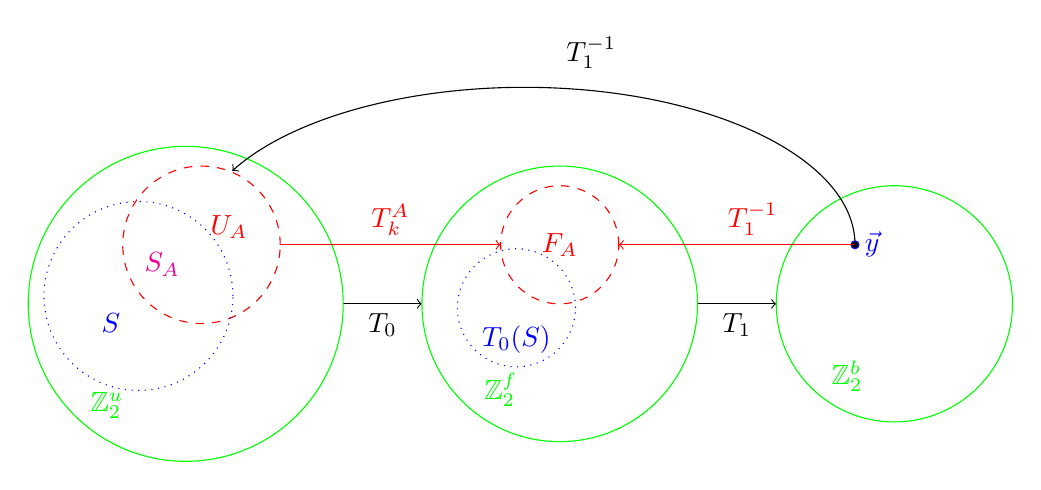
\begin{tikzpicture}
		\draw[->] (4,2) -- (5,2) node[left=0.5cm,below] {$T_0$};
		\draw[green] (2,2) circle (2cm) node[left=1cm,below=1cm] {$\binvecspace{u}$};
		\draw[green] (6.75,2) circle (1.75cm) node[left=0.75cm,below=0.75cm] {$\binvecspace{f}$};
		\draw[->] (8.5,2) -- (9.5,2) node[left=0.5cm,below] {$T_1$};
		\draw[green] (11,2) circle (1.5cm) node[left=0.6cm,below=0.6cm] {$\binvecspace{b}$};
		
		\draw[blue] (10.5,2.75) circle (0.05cm) [fill=black] node[anchor=west] {$\vec{y}$};
		\draw[->,red] (10.5,2.75) -- (7.5,2.75) node[left=-1.7cm,above] {$T_1^{-1}$};
		\draw[dashed,red] (6.75,2.75) circle (0.75cm)  node[] {$F_A$};
		\draw[dotted,blue] (6.2,1.95) circle (0.75cm)  node[left=0cm,below=0.1cm] {$T_0(S)$};

		\draw[dashed,red] (2.2,2.75) circle (1cm)  node[left=-0.35cm,below=-0.5cm] {$U_A$};
		\draw[dotted,blue] (1.4,2.1) circle (1.2cm)  node[left=0.35cm,below=0.1cm] {$S$};
		
		\draw[magenta] (1.7,2.5) node[] {$S_A$};
		

		\draw[->] (10.5,2.75) arc (0:152:4.2cm and 2cm) node[below=-1.5cm,left=-5cm] {$T_1^{-1}$};
		
		
		\draw[->,red] (3.2,2.75) -- (6,2.75) node[left=1.4cm,above] {$T_k^A$};
	\end{tikzpicture}
\end{center}
\end{figure}

\begin{figure}
	\caption{Factorisation of $T$ when event $E_2(S, T_0, T_1)$ occurs, i.e. $F_A \subseteq T_0(S)$.}
	\label{fig-factorisation-e2}

\begin{center}
	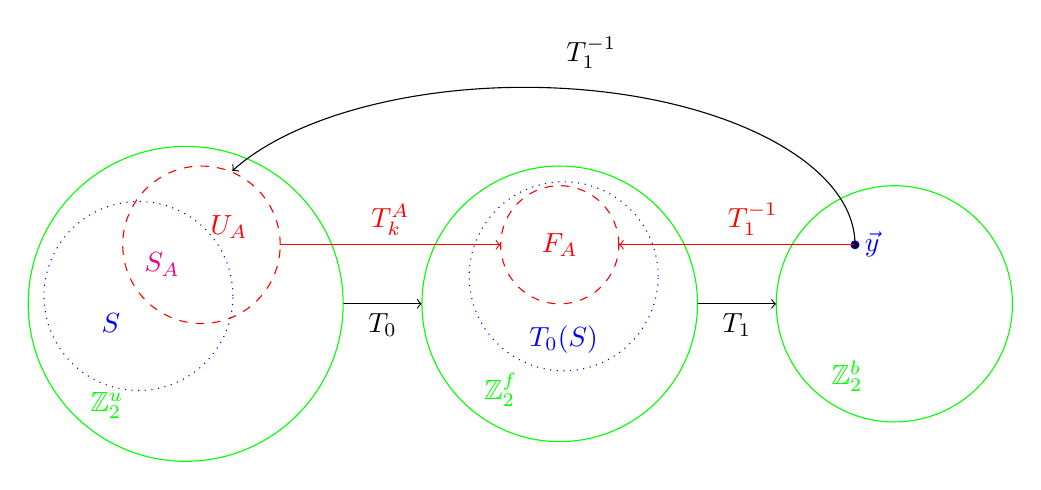
\begin{tikzpicture}
		\draw[->] (4,2) -- (5,2) node[left=0.5cm,below] {$T_0$};
		\draw[green] (2,2) circle (2cm) node[left=1cm,below=1cm] {$\binvecspace{u}$};
		\draw[green] (6.75,2) circle (1.75cm) node[left=0.75cm,below=0.75cm] {$\binvecspace{f}$};
		\draw[->] (8.5,2) -- (9.5,2) node[left=0.5cm,below] {$T_1$};
		\draw[green] (11,2) circle (1.5cm) node[left=0.6cm,below=0.6cm] {$\binvecspace{b}$};
		
		\draw[blue] (10.5,2.75) circle (0.05cm) [fill=black] node[anchor=west] {$\vec{y}$};
		\draw[->,red] (10.5,2.75) -- (7.5,2.75) node[left=-1.7cm,above] {$T_1^{-1}$};
		\draw[dashed,red] (6.75,2.75) circle (0.75cm) node[] {$F_A$};
		\draw[dotted,blue] (6.8,2.35) circle (1.2cm)  node[left=0cm,below=0.5cm] {$T_0(S)$};

		\draw[dashed,red] (2.2,2.75) circle (1cm)  node[left=-0.35cm,below=-0.5cm] {$U_A$};
		\draw[dotted,blue] (1.4,2.1) circle (1.2cm)  node[left=0.35cm,below=0.1cm] {$S$};

		\draw[->] (10.5,2.75) arc (0:152:4.2cm and 2cm) node[below=-1.5cm,left=-5cm] {$T_1^{-1}$};
		
		\draw[magenta] (1.7,2.5) node[] {$S_A$};
				
		\draw[->,red] (3.2,2.75) -- (6,2.75) node[left=1.4cm,above] {$T_k^A$};
	\end{tikzpicture}
\end{center}
\end{figure}

\begin{corollary}
\label{corollary-e1-e2}
For each $\epsilon > 0$ there is $c_\epsilon > 0$ such that if $l \geq c_\epsilon (f - b)2^{f-b}$, then
\[
\probs{T \in_U \linearmaps{u}{b}}{E_1} \leq \frac{1}{1 - \epsilon}\probs{T_0 \in_U \linearmaps{u}{f}, T_1 \in_U \surjectivelinearmaps{f}{b}}{E_2}
\]
\end{corollary}
\begin{proof}
From Lemma~\ref{lemma-e1-e2} we get that $1 - \epsilon \leq \prob{E_2 | E_1}$.
This bound holds for arbitrary fixed $T$ and $T_1$ with the uniform choice of $T_k$.
Hence it must also hold for any random choice of $T$ and $T_1$, in our case it is the uniform choice.
Further from the definition of conditional probability we get that $1 - \epsilon \leq \frac{\prob{E_2}}{\prob{E_1}}$ where both probabilities are taken in the probability space of uniform choice of $T$ and $T_1$.
Recall that the definition of $E_1$ does not take into account $T_1$.
Considering that the uniform choice of $T_0$ and $T_1$ leads to the uniform choice of $T$ and $T_1$ and vice-versar we obtain the wanted statement.
\end{proof}

Now we switch to estimating the probability of occurrence of $E_2$. 
Since we assume that $|S| = n$, instead of $n \log n$ as it is in \cite{alonetal}, we now start to differentiate from the original proof.
The substantial advantage is that we can start using the following lemma for $f > b$ instead of $f > b + \log b$ as it is in Proposition~3.1 of \cite{alonetal}.
On the other hand since our estimate depends on $b$ the calculation becomes a tiny bit more complicated than the one from the original article.

\begin{lemma}
\label{lemma-bound}
If $S \subseteq \binvecspace{u}$, $|S| = 2^b$ and $\mu = \frac{|S|}{|\binvecspace{f}|} = 2^{b - f} < 1$, then
\[
\probs{T_0 \in_U \linearmaps{u}{f}, T_1 \in_U \surjectivelinearmaps{f}{b}}{E_2(S, T_0, T_1)} \leq \mu ^ {-\log b - \log \mu + \log \log \mu^{-1}}.
\]
\end{lemma}
\begin{proof}
Observe that it is possible to restate $E_2(S, T_0, T_1)$ as $T_1(\binvecspace{f} - T_0(S)) \neq \binvecspace{b}$. 
For more details check Figure~\ref{fig-factorisation-e2}.
Occurrence of $E_2(S, T_0, T_1) \equiv \exists \vec{y} \in \binvecspace{b} \colon T_1^{-1}(y) \subseteq T_0(S)$ is equivalent to $T_1(\binvecspace{f} - T_0(S))$ not containing $\vec{y}$, i.e. $E_2(S, T_0, T_1) \equiv \exists \vec{y} \colon \vec{y} \not\in T_1(\binvecspace{f} - T_0(S))$.

We use Theorem~\ref{theorem-prob-bound} to estimate $\probs{T_1\in_U \surjectivelinearmaps{f}{b}}{T_1(\binvecspace{f} - T_0(S)) \neq \binvecspace{b}} \leq \alpha ^ {f - b - \log b + \log \log \alpha^{-1}}$ where $\alpha = 1 - \frac{|\binvecspace{f} - T_0(S)|}{|\binvecspace{f}|} \leq \frac{|T_0(S)|}{2^f} \leq \frac{|S|}{2^f} \leq \mu$.
Since the function $\alpha ^ {f - b - \log b + \log \log \alpha^{-1}}$ is increasing w.r.t. $\alpha$ in $(0, 1)$ we get that
$
\prob{E_2(S, T_0, T_1)} \leq \mu ^ {-\log \mu - \log b + \log \log \mu^{-1}}.
$
\end{proof} 

Now we compute the tail distribution of the variable $\lbin{T}{S}$ using the estimate from Lemma~\ref{lemma-bound} which in turns directly gives Theorem~\ref{theorem-n-to-n}.

\begin{theorem}
\label{theorem-prob-distribution-bound}
Let $r > 4$. Then
\[
\probs{T \in_U \linearmaps{u}{b}}{\lbin{T}{S} \geq 2 c_\epsilon r} \leq \frac{1}{1 - \epsilon}\left(\frac{\log r}{r}\right)^{-\log b - \log \frac{\log r}{r} + \log \log \frac{r}{\log r}}.
\]
\end{theorem}
\begin{proof}
In this proof we fix $f = \lfloor b + \log r - \log \log r + 1 \rfloor$ and $l = 2c_\epsilon r$.

To bound the probability of $E_1(S, T, 2 c_\epsilon r)$, i.e. $\lbin{T}{S} \geq 2 c_\epsilon r$, we first obtain an estimate on $\prob{E_2(S, T_0, T_1)}$ using the factor space $\binvecspace{f}$. 

The choice of $f$ meets the requirement $f > b$ of Corollary~\ref{corollary-e1-e2} and Lemma~\ref{lemma-bound} which means that $\surjectivelinearmaps{f}{b}$ is nonempty.

To use Corollary~\ref{corollary-e1-e2} we have to verify that $l \geq c_\epsilon (f - b)2^{f - b}$.
Since we assume that $r \geq 4$ we have $(f - b)2^{f - b} \leq (\log r - \log \log r + 1)2^{\log r - \log \log r + 1} \leq \frac{2r(\log r - \log \log r + 1)}{\log r} \leq 2r$ and this requirement is thus met.

From Lemma~\ref{lemma-bound}, the fact that $\mu = 2^{b - f} \leq \frac{\log r}{r}$ and that $f(\mu) := \mu ^ {- \log b + \log \mu^{-1} + \log \log \mu^{-1}}$ is increasing in $(0, 1)$ it follows that $\prob{E_2(S, T_0, T_1)} \leq f(\mu) \leq f(\log r/r)$.
Bounding $\prob{E_1}$ using Corollary~\ref{corollary-e1-e2} yields the statement.
\end{proof}

The main advantage is that the proven estimate becomes less than one for $r \approx b$. 
This is enabled by the possibility of having smaller factor spaces, since $f$ is chosen closer to $b$.

\begin{proof}[Proof of Theorem~\ref{theorem-n-to-n}]
We tear $\sum_{l = 1}^{n} \probs{T\in_U\linearmaps{u}{b}}{\lbin{T}{S} \geq l}$ into two sums according to $l$ being lower or greater than $8c_\epsilon \log n$.
We show that the probability of having a chain longer then $2 c_\epsilon r$ is bounded from above by $\frac{r^{-1.5}}{1-\epsilon}$ when $r \geq 4\log n$.
Using the previous fact we conclude that $\sum_{l = 8c_\epsilon \log n}^{n} \probs{T\in_U\linearmaps{u}{b}}{\lbin{T}{S} \geq l} = \frac{O(1)}{1-\epsilon}$ and $\sum_{l = 1}^{8c_\epsilon \log n} \probs{T\in_U\linearmaps{u}{b}}{\lbin{T}{S} \geq l} \leq 8c_\epsilon \log n$.

It remains to show that for $r \geq 4 \log n$ the estimate of the previous theorem is below $\frac{r^{-1.5}}{1-\epsilon}$.
Assuming $r \geq 4 \log n$ we estimate the exponent from Theorem~\ref{theorem-prob-distribution-bound} as
\[
-\log b - \log \log r + \log r + \log (\log r - \log \log r) \geq -\log \log r + 2 + \log \left(\frac{3\log r}{4}\right) = \log(3).
\]
Hence for $r \geq 4\log n$ we may conclude that $\prob{\lbin{T}{S} \geq 2c_\epsilon r} \leq \frac{\left(\frac{\log r}{r}\right)^{\log 3}}{1-\epsilon} \leq \frac{r^{-1.5}}{1-\epsilon}$.
\end{proof}

\section{A Special Case When $S$ is a Vector Subspace}

Let us note that when $S$ is a subspace of the universe, then the expected size of the largest bin is constant.

\begin{theorem}
Let $b, u \in \mathbb{N}$ and $v_1, \dots, v_b \in \mathbb{Z}_2^u$ be linearly independent. Then \[ \expects{h \in_U \linearmaps{u}{b}}{\lbin{h}{\operatorname{Span}(v_1, \dots, v_b)}} = O(1) .\]
\end{theorem}
\begin{proof}
We first notice that the bins have a simple structure -- all of them are formed by elements which are affine subspaces of the universe.
This means that the non-empty bins have the same size.
In addition the bin $\vec{0}$ in $\binvecspace{b}$ is always non-empty is a largest bin of expected constant size.

For convenience put $S = \operatorname{Span}(v_1, \dots, v_b)$. 
We show that each non-empty bin created by a transformation $h$ is formed by balls from an affine subspace of $S$ and has the size of the kernel of $h$.
From this it follows that $\expect{\lbin{h}{S}} = \expect{\bin{h}{S}{0}} = O(1)$.

Without loss of generality assume that $v_1, \dots, v_k$ are the vectors forming the kernel of $h$, i.e. $h(v_i) = 0$ where $i \in \{1, \dots, k\}$.
If $h(v) = y$ for some $v \in S$, then $h^{-1}(y) \cap S = v + \operatorname{Span}(v_1, \dots, v_k)$.
Hence for each $y \in \mathbb{Z}_2^b$ it holds hat $|h^{-1}(y) \cap S| = 0 \vee |h^{-1}(y) \cap S| = 2^k$.
Thus the sizes of all the non-empty bins are the same and are equal to $\bin{h}{S}{0}$.
\end{proof}

\section{Acknowledgement}

% TODO: UTF-8 not working?

I would like to thank Michal Koucky and Vaclav Koubek for many advices and  time spent helping me with creating this article.

\begin{thebibliography}{32}
\bibitem{alonetal}
N. Alon, M. Dietzfelbinger, P. B. Miltersen, E. Petrank and G. Tardos
\newblock Linear Hash Functions
\newblock J. {ACM}, 46. pages 667--683, 1999

\bibitem{siegel}
A. Siegel. 
\newblock On universal classes of extremely random constant-time hash functions
\newblock SIAM Journal on Computing, 33(3). pages 505--543 (electronic), 2004

\bibitem{celisetal}
L.E. Celis, O. Reingold, G. Segen and U. Wieder
\newblock Balls and Bins: Smaller Hash Families and Faster Evaluation
\newblock Foundations of Computer Science (FOCS), 2011 IEEE 52nd Annual Symposium, pages 599 -- 608, 2011

\bibitem{linear-probing}
A. Pagh, R. Pagh and M. Ruzic
\newblock Linear Probing with Constant Independence
\newblock Proceedings of the Thirty-ninth Annual ACM Symposium on Theory of Computing (STOC), pages 318--327, 2007 

\bibitem{mitzenmacher-cuckoo} 
A. Kirsch, M. Mitzenmacher and U. Wieder
\newblock More Robust Hashing: Cuckoo Hashing with a Stash
\newblock {SIAM} J. Comput., Vol. 39, pages 1543--1561, 2009
               
\bibitem{dietzfelbinger-cuckoo}
M. Aum{\"{u}}ller, M. Dietzfelbinger and P. Woelfel
\newblock Explicit and Efficient Hash Families Suffice for Cuckoo Hashing with a Stash
\newblock Algorithms - {ESA} 2012 - 20th Annual European Symposium, Ljubljana, Slovenia, September 10-12, 2012. Proceedings

% \bibitem{cw}
% J.L. Carter, and M.N. Wegman. 
% \newblock Universal Classes of Hash Functions.
% \newblock Journal of Computer and System Sciences, 18. pages 143--154, 1979.


% \bibitem{azar}
% Y. Azar, A. Broder, A. Karlin, and E. Upfal
% \newblock Balanced allocations.
% \newblock SIAM Journal on Computing, 29(1). pages 180--200, 1999.

% \bibitem{vocking}
% B. V\"{o}cking
% \newblock How asymmetry helps load balancing.
% \newblock In Proceedings of the Fortieth Annual Symposium on Foundations of Computer Science. pages 131--140, 1999.
\end{thebibliography}

\end{document}


 
